\documentclass[a4paper]{scrreprt}

\usepackage[german]{babel}
\usepackage[utf8]{inputenc}
\usepackage[T1]{fontenc}
\usepackage{ae}
\usepackage[bookmarks,bookmarksnumbered]{hyperref}
\usepackage{graphicx}
\usepackage[toc]{glossaries}
% \usepackage{float}
\graphicspath{ {Images/} }
\setcounter{secnumdepth}{5}
\makeglossaries

\begin{document}
    \newglossaryentry{Versuchsleiter}{name=Versuchsleiter, description={jemand, unter dessen Leitung ein Versuch durchgeführt wird}}
    \newglossaryentry{Proband}{name=Proband, description={Versuchs-, Testperson}}
    \newglossaryentry{Web-Interface}{name=Web-Interface, description={Benutzeroberfläche, die man in einem Web-Browser nutzen kann}}

    \begin{flushright}
        
\includegraphics[scale = 0.7]{kit-logo.jpg}\\[0.5cm]
        % 
\includegraphics[scale = 1]{teco.jpg}
    \end{flushright}
    % 
\includegraphics[scale = 0.5]{kit-logo.jpg} \hspace{4cm} 
\includegraphics[scale = 1]{teco.jpg}
    \vspace*{2cm}

    \begin{center} \large

        Praxis der Softwareentwicklung
        \vspace * {1.5cm}

        \textbf{\huge Mind Rate}
		
        \vspace*{1cm}
		
        {\Large Ein interaktives Werkzeug f\"ur Studie nach Experience-Sampling-Method (ESM)}

        \vspace*{1cm}

        \textbf{\Large Pflichtenheft}
        \vspace*{2cm}

        Shanshan Du, Yi Ge, Renhan Lou, Ruoheng Ma, Haobin Tan
        \vspace*{1cm}

        02. Dezember 2016
        \vspace*{2.5cm}


        Betreuung: Anja Exler, Dr. Andrea Schankin, Erik Pescara\\[1cm]
        Technology f\"ur Pervasive Computing\\[0.5cm]
        Karlsruher Institut für Technologie
    \end{center}

    \tableofcontents

    \chapter{Zielbestimmung}
    % Dieses Kapitel dient der Bestimmung von Zielen und nicht für deren Verwendung
    % notwendige Funktionen.
        Die Firma soll durch das Produkt in die Lage versetzt werden, psychologische Studien nach Experience-Sampling-Method (ESM) durchzuf\"uhren und Feedbacks der Studien zu erhalten.\\

        \noindent Das Produkt besteht aus zwei Teilsysteme: ein Web-Interface f\"ur den Versuchsleiter und eine Android-Anwendung f\"ur die Probanden.


        \section{Musskriterien}
            % Musskriterien: Für das Produkt unabdingbare Leistungen, die in jedem Fall
            % erfüllt werden müssen \footnote{gezwungen sein, etwas zu tun (Dies ist eine
            % beispielhafte Fußnote).}. Das System ist ohne diese Funktionen für seinen
            % gedachten Zweck nicht einsetzbar.
            \vspace*{0.3cm}

            \subsection{Web-Interface f\"ur Versuchsleiter}
                \vspace*{0.2cm}

                \subsubsection{Verwalten von Teilnehmer der Untersuchung}
                    \begin{itemize}
                        \item Probandsstatus erfassen (z.B. Proband-ID, Alter, Geschlecht, Beruf)
                        \item Anmelden f\"ur Durchf\"uhrung der Untersuchung
                    \end{itemize}

                \subsubsection{Verwalten der Frageb\"ogen}
                    \begin{itemize}
                        % \item Ausw\"ahlen von Prob\"ande nach verschiedenen Kriterien vor Erstellung der Frageb\"ogen
                        \item Erstellen, \"Andern von Untersuchungsfragen f\"ur unterschiedliche Probandsgruppe
                        \item Erstellen, \"Andern von Scale und Optionen der Antworten
                        \item Setzen, \"Andern von G\"ultigkeitszeitbereich der Untersuchungsfragen
                        \item Setzen, \"Andern von H\"aufigkeit der Notifikationen zur Antworten
                        % \item Senden von Feedback und Motivation zu Probanden
                    \end{itemize}

                \subsubsection{Erfassen von Ergebnisse der Untersuchung}
                    \begin{itemize}
                        \item Besichtigen von Antwortsstatus
                        \item Exportieren von Daten
                    \end{itemize}
            \vspace*{2cm}

            \subsection{Android-Anwendung f\"ur Probanden}
                \vspace*{0.2cm}

                \subsubsection{Anmelden f\"ur Beteiligung der Studie}

                \subsubsection{Antwort auf Untersuchungsfragen}
                    \begin{itemize}
                        \item regelm\"assige Notifikation zur Antworten
                        \item Untersuchungsfragen beantworten
                    \end{itemize}

                \subsubsection{Verwalten von Antworten}
                    \begin{itemize}
                        \item lokales Speichern von Antworten
                        \item Protokollieren von Zeitpunkt der Antwort
                        \item Hochladen von Antworten auf den Server
                    \end{itemize}

                \subsubsection{Zurgreifen einiger Sensoren von Handy}
                    \begin{itemize}
                        \item Zugreifen von Temperatursensor
                        \item Zugreifen von GPS
                    \end{itemize}
                \vspace*{0.5cm}


        \section{Wunschkriterien}
            \vspace*{0.3cm}
            % Kannkriterien: Die Erfüllung der Kannkriterien ist erwünscht, jedoch nicht
            % unbedingt notwendig. Sie sollten nur angestrebt werden, falls noch ausreichend
            % Kapazitäten vorhanden sind.

            \subsection{Web-Interface f\"ur Versuchsleiter}
                \begin{itemize}
                     % \item Emailbest\"atigugn beim (erfolgreichen) Anmelden
                    \item Erm\"oglichen von ``angemeldet bleiben"
                    \item Erzeugen von verschiedenen (Statistik-)Diagramme f\"ur hochgeladene Daten (z.B. S\"aulendiagramm, Kreisdiagramm)
                    \item Unterst\"utzen von unterschiedlichen Sprachen

                \end{itemize}

            \subsection{Android-Anwendung f\"ur Probanden}
                \begin{itemize}
                    \item Erm\"oglichen von ``angemeldet bleiben"
                    \item Unterst\"utzen von unterschiedlichen Sprachen
                    \item Wechseln von Theme der Anwendung
                \end{itemize}
                \vspace*{0.5cm}


        \section{Abgrenzungskriterien}
            % Abgrenzungskriterien: Diese Kriterien sollen bewusst nicht erreicht werden.
            \begin{itemize}
                \item Keine verteilte Datenbank, keine Echtzeitanforderungen, keine synchronisierten Datenbankzugriffe
                \item Keine Unterst\"utzung f\"ur iOS
            \end{itemize}

    \chapter{Produkteinsatz}
        Das Produkt dient zur Sammlung der Versuchsdaten aus ESM-Versuchen. Damit bietet sie für Versuchsleiter eine Lösung, ESM-Versuchen durchzuführen. Diese Tätigkeit soll zusätzlich im Internet und auf dem Smartphone möglich sein.

        \section{Anwendungsbereiche}
            \begin{itemize}
                \item Akademischer / Sozialwissenschaftlicher Anwendungsbereich
                \item Statistischer Anwendungsbereich
                \item Geschäftlicher Anwendungsbereich
            \end{itemize}

        \section{Zielgruppen}
            \begin{itemize}
                \item Versuchsleiter eines ESM-Versuchs
                \item Teilnehmer des Versuchs
            \end{itemize}

        \section{Betriebsbedingungen}
            \begin{itemize}
                \item Versuchsleiter: Büroumgebung
                \item Versuchsteilnehmer: im alltäglichen Leben aufs Smartphone
                \item Betriebszeit rund um die Uhr, läuft unbeaufsichtigt
            \end{itemize}

    \chapter{Produktumgebung}
        Eine Client-Server Architektur mit 2 Client-Typen: ein Web-Interface für Versuchsleiter und eine Android-App für Probanden

        \section{Software}
            \begin{itemize}
                \item Serverseite
                    \begin{itemize}
                        \item  Läuft auf Linux
                        \item Alle Softwares der Serverseite werden durch Docker verpackt
                        \item Datenbank: SQLite, verwaltet durch das Django-Framework
                        \item Programmiersprache: Python 3
                        \item Web server: Nginx
                    \end{itemize}
                \item Clientseite
                    \begin{itemize}
                        \item Web-Interface\\
                             Web-Browser, Referenzstandard Google Chrome 54
                        \item  Android-App\\
                             Android, Referenzstandard Android 5.1.1 Lollipop
                    \end{itemize}
            \end{itemize}

        \section{Hardware}
            \begin{itemize}
                \item Serverseite\\
                    Leistungsstarke Standardrechner
                \item  Web-Interface\\
                    Standardrechner (für Web-Browser)
                \item Android-App\\
                    Standardsmartphone
            \end{itemize}

    \chapter{Funktionale Anforderungen}

		\section{Web-Interface}
	        \begin{itemize}
	            \item \textbf{/F10/Registrieren oder Anmelden der Leiter}
		
	            	\par \textbf{Ziel: }Registrieren oder Anmelden der Versuchsleiter in der Web-Verwaltungssystem
	            	\par \textbf{Vorbedingung (Registrieren): }-keine-
	            	\par \textbf{Vorbedingung (Anmelden): }Ein Konto des Leiters soll vorhanden sein.
	            	\par \textbf{Nachbedingung (erfolgreiches Registrieren): }Der Leiter bekommt eine Bestätigungsmail und kann sich mit dem neu erzeugten Konto anmelden.
	            	\par \textbf{Nachbedingung (erfolgreiches Anmelden): }Der Leiter ist in der Verwaltungssystem angemeldet und kann seine Versuche verwalten.
	            	\par \textbf{Nachbedingung (Fehlschlag): }Der Leiter bleibt unangemeldet.
	            	\par \textbf{Akteure: }Versuchsleiter
	            	\par \textbf{Auslösendes Ereignis: }Der Leiter busucht die Webseite dieses Online-Verwaltungssystems.
	            	\par \textbf{Beschreibung: }
		            	\begin{enumerate}
		            		\item Beim Registrieren soll der Leiter eine gültige Email-Adresse als Konto-Name und ein gültiges Passwort eintragen. Diese Daten werden von dem Datenbank gespeichert und der Server erzeugt ein neues Konto. Danach empfängt der Leiter eine Bestätigungsmail und kann sich mit dem neuen Konto anmelden.
			            	\item Beim Anmelden soll der Leiter die registrierte Email-Adresse und sein Passwort eingeben. Wenn die Email-Adresse und das Passwort stimmen überein, dann wird der Leiter in die Verwaltungsseite weitergeleitet.
		            	\end{enumerate}
	            	\par \textbf{Erweiterung: }
	            	\par \textbf{Alternativen: }
	            	
	            \item \textbf{/F20/Vergessenes Passwort neu zu setzen}
	
	            \par \textbf{Ziel: }Vergessenes Passwort neu zu setzen
	            \par \textbf{Vorbedingung: }-keine-
	            \par \textbf{Nachbedingung (Konto vorhanden): }Der Leiter bekommt eine Bestätigungsmail mit einem Link. Wenn der Leiter auf den Link klickt, wird er in die Passwort-Setzen-Seite geleitet und kann da sein neues Passwort eingeben.
	            \par \textbf{Nachbedingung (Konto nicht vorhanden): }Eine Fehleranzeige mit Wörtern ``Konto existiert nicht'' kommt in dem Browser auf.
	            \par \textbf{Akteure: }Versuchsleiter
	            \par \textbf{Auslösendes Ereignis: }Der Leiter vergisst sein Passwort.
	            \par \textbf{Beschreibung: }
	            \begin{enumerate}
	            	\item Klicken auf ``Passwort Vergesse''
	            	\item Email-Adresse eingeben
	            	\item Der Versuchsleiter empfängt ein Bestätigungsemail mit einem Link
	            	\item Durch den Link ist der Versuchsleiter in die “Passwort neu setzen” Seite weitergeleitet
	            	\item Neues Passwort eingeben
	            	\item Sein neues Passwort wird in dem Datenbank gespeichert
            	\end{enumerate}
	            \par \textbf{Erweiterung: }
	            \begin{itemize}
		            \item Falls das Konto nicht vorhanden ist, kommt eine Fehleranzeige sofort in dieser Seite auf. Sonst sendet der Server eine Bestätigungsmail mit einem Link zu der Email-Adresse. Durch diesen Link wird der Leiter in die Passwort-Setzen-Seite geleitet und kann er da sein neues Passwort eingeben.
	            \end{itemize}
	            \par \textbf{Alternativen: }
	
	            \item \textbf{/F30/Verwaltung der Fragen }
	            \par \textbf{Ziel: }Erstellung der Fragen in einem Versuch
	            \par \textbf{Vorbedingung: } Angemeldet in dem Verwaltungssystem
	            \par \textbf{Nachbedingung (Erfolg): }Eine neue Frage wird erstellt.
	            \par \textbf{Nachbedingung (Fehlschlag): }Eine neue Frage wird nicht erstellt
	            \par \textbf{Akteure: }Versuchsleiter
	            \par \textbf{Auslösendes Ereignis: }Der Versuchsleiter vesucht, den ``neu'' Button auf der Webseite zu klicken
	            \par \textbf{Beschreibung: }
	            \begin{enumerate}
	            	\item Verwaltung des Versuchs
	            	\par Der Versuchsleiter wählt zuerst einen Versuch aus oder erstellt er einen neuen Versuch. Zudem gehört die neue Frage.
	            	\item Erstellung der Fragen
	            	\par Der Versuchsleiter entscheidet sich die Fragenart und Antwortart. Dann soll der Versuchsleiter auch konkrete Frage eingeben.
	            	\item Zeiteinstellung
	            	\par Der Versuchsleiter stellt die Antwortfrist und die Push-Zeit der Frage ein.
	            	\item Hardwareunterstützung(bzw. Sensoren)
	            	\par Der Versuchsleiter fügt die Sensoren hinzu. Die Sensoren sollen während der Antwort von dem Proband benutzt werden.
                    \item Verwaltung der Beziehungen zwischen Fragen
                    \par Der Versuchsleiter entscheidet sich, welche Frage und welche Option das auslösende Ereignis dieser Frage ist.
	            	\item Abschicken und Stornieren
	            	\par Der Versuchsleiter entscheidet sich, ob er die Frage eines Versuchs hinfügt oder storniert.
	            \end{enumerate}
	            \par \textbf{Erweiterung: }
	            \begin{enumerate}
	            	\item Es gibt fünf Fragenarten. Die sind jeweils ``Single-Choice-Frage'', ``Multiple-Choice-Frage'', ``Skala mit Stufen Frage'', ``Skala ohne Stufe Frage'' und ``Offene Frage''.
	            	\item a. Der Versuchsleiter kann sich entscheiden,ob diese Frage eine Frist hat. Falls ja, soll der Versuchsleiter  einen exakten Zeitraum auswählen.
	            	\par b. Der Versuchsleiter soll eine Push-Zeit für diese Frage hinfügen. Er kann sich noch entscheiden, ob die Push-Zeit dem Zeitraum des Probandes entsprechend ist.
	            	\item Der Versuchsleiter kann sich entscheiden, wie viele und welche Sensoren benutzt werden sollen. Wenn ein Sensor hingefügt ist, soll der Versuchsleiter einen Zahlenwert (z. B. Temperatur) für den Sensor eingeben.
	            	\item Zwei Buttons ``submit'' und ``cancel'' sind auf der Webseite vorhanden.
                    \item Es ist nicht notwendig, die Probanden den Fragebogen sequenziell zu antworten. Der Versuchsleiter kann sich entscheiden, welche Fragen die Probanden antworten müssen und welche Fragen ein auslösende Ereignis haben.
	            \end{enumerate}
	            \par \textbf{Alternativen: }
	
	
	            \item /F40/ \textbf{Antwortsstatus besichtigen}
	            \par \textbf{Ziel: }Besichtigung der Antwortsstatus
	            \par \textbf{Vorbedingung: }Der Versuchsleiter ist angemeldet.
	            \par \textbf{Nachbedingung : }Der neue Antwortsstatus eines Fragebogens (z.B. Verteilung der Antwroten, Anzahl der beantworteten Probanden) ist besichtgbar.
	            \par \textbf{Nachbedingung (Fehlschlag): }Der neue Antwortsstauts wird nicht gezeigt.
	            \par \textbf{Akteure: }Versuchsleiter
	            \par \textbf{Auslösendes Ereignis: }Der Versuchsleiter kann die \"Ubersicht von Antworten des aktuellen Fragebogens sehen.
	            \par \textbf{Beschreibung: }
	            \begin{enumerate}
	            	\item Klicken von Button ``View answers''
	            	\item Zeigen der \"Ubersicht von allen Antwort beim erfolgreichen Anmelden
	            	\item Erfassen von Antwortsstatus nach Bedarf und eingegebener Kriterien
	            	\item Laden des neuen Antwortsstatus beim Klicken von Button ``Refresh''
	            \end{enumerate}
	            \par \textbf{Erweiterung: }
	            \par \textbf{Alternativen: }
	            \begin{figure}[ht]
	            	% \raggedleft
	            	\centering
	            	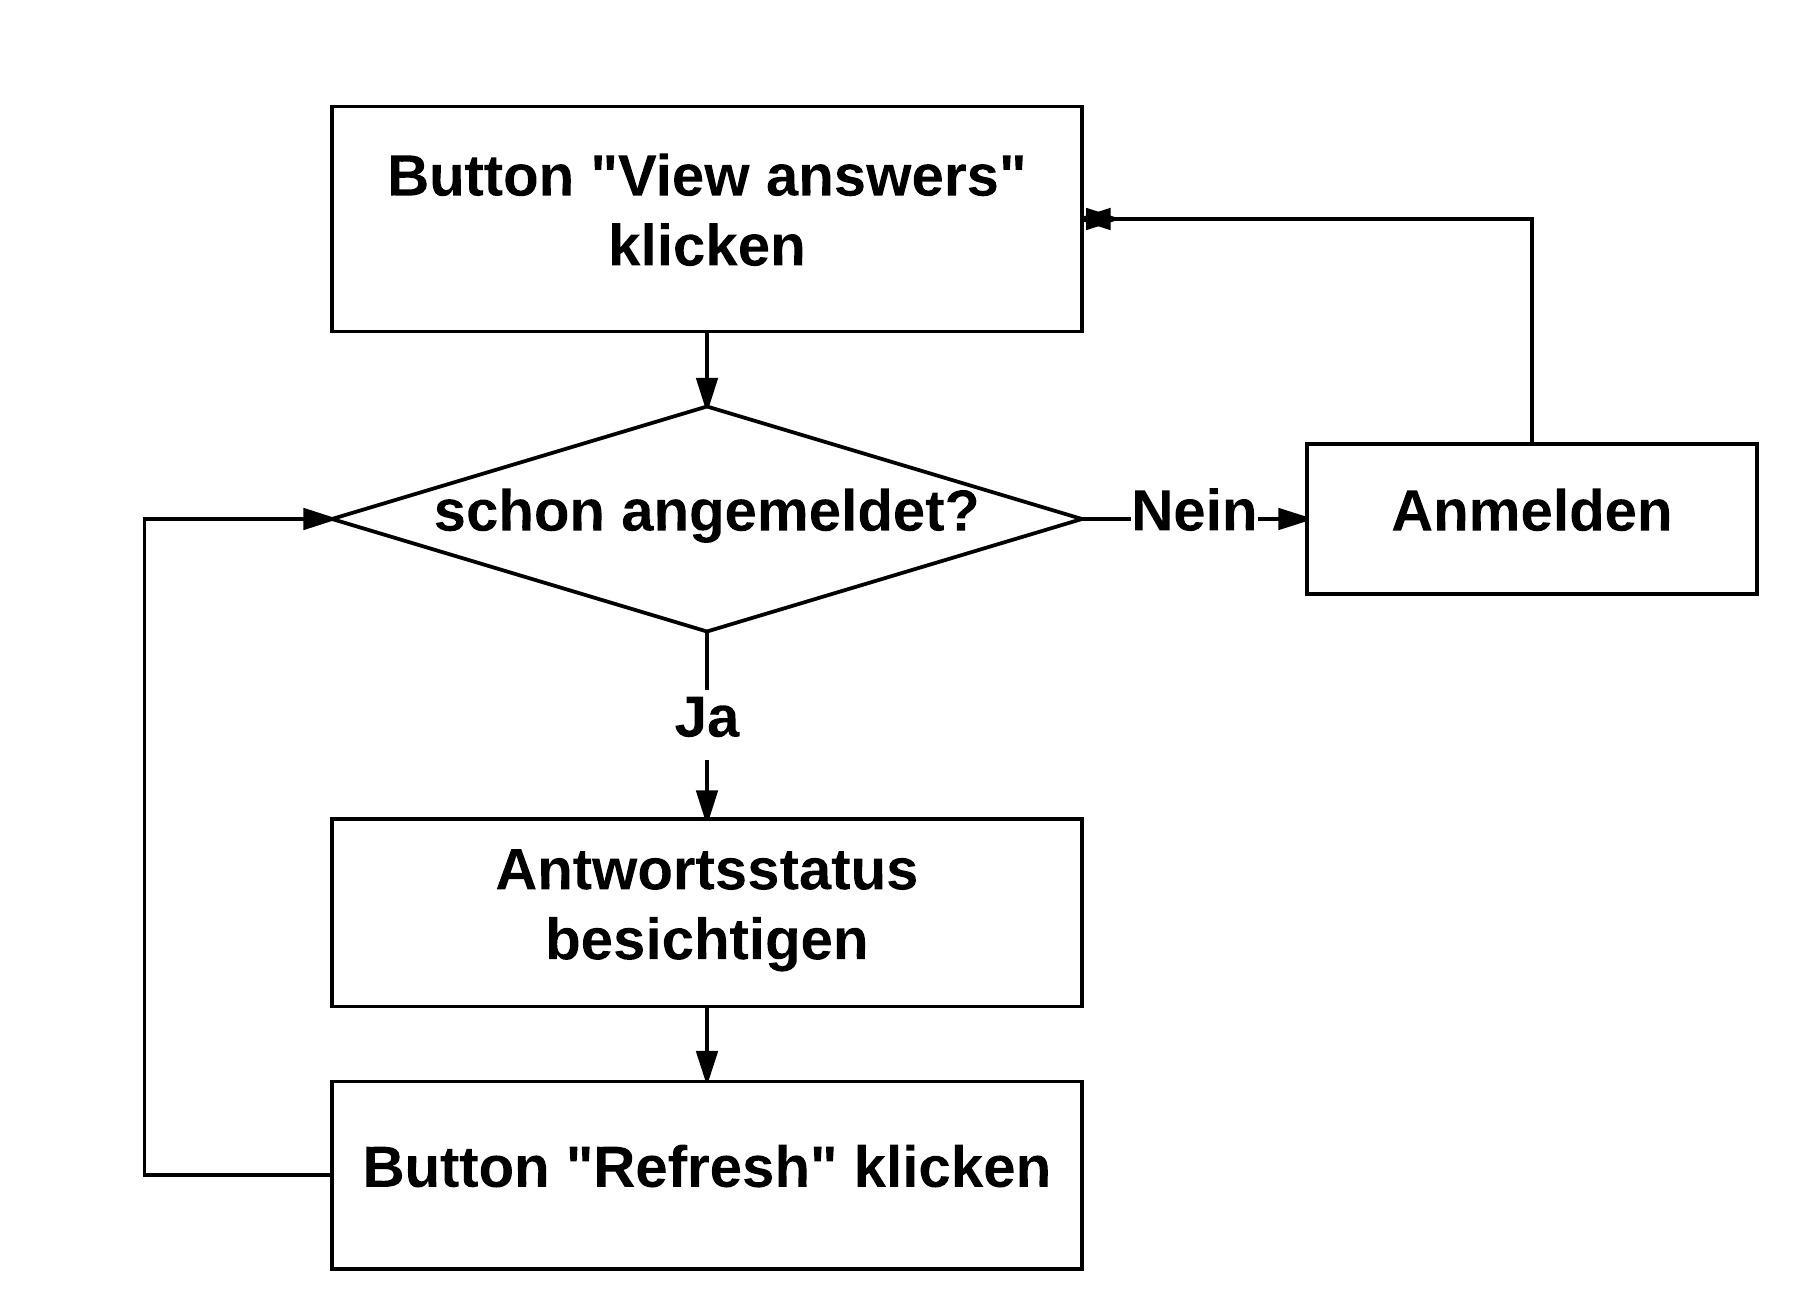
\includegraphics[scale=0.8]{Antwortsstatus_besichtigen.jpeg}
	            	\caption{Antwortsstatus besichtigen}
	            \end{figure}
	
	
	            \item /F45/ \textbf{Feedback (Motivation) senden}
	            \par \textbf{Ziel: }Senden von Feedbacks (Motivation), um Proband zu motivieren, die Studie weiter zu beteiligen.
	            \par \textbf{Vorbedingung: }Der Versuchsleiter ist angemeldet.
	            \par \textbf{Nachbedingung : }Jeder Proband erhalten Motivation vom Versuchsleiter.
	            \par \textbf{Nachbedingung (Fehlschlag): }Die Proband erhalten keine Feedbacks.
	            \par \textbf{Akteure: }Versuchsleiter
	            \par \textbf{Auslösendes Ereignis: }Alle Probanden erhalten die von Versuchsleiter geschriebene Motivation.
	            \par \textbf{Beschreibung: }
	            \begin{enumerate}
	            	\item Klicken von Button ``Send Feedback / Motivation''
	            	\item Schreiben von Feedback (Motivation)
	            	\item Klicken von Button ``Send'', um die Feedbacks an allen Probanden zu senden.
	            \end{enumerate}
	            \par \textbf{Erweiterung: }
	            \par \textbf{Alternativen: }
	            	
	            \item \textbf{/F50/Exportieren von Daten}
	
	            \par \textbf{Ziel: }Exportieren von Antworten und statistischen Daten
	            \par \textbf{Vorbedingung: }Angemeldet in dem Verwaltungssystem
	            \par \textbf{Nachbedingung (Erfolg): }Die den Versuchen zugehörigen Daten werden in CSV-Format exportiert.
	            \par \textbf{Nachbedingung (Fehlschlag): }Die den Versuchen zugehörigen Daten werden nicht exportiert.
	            \par \textbf{Akteure: }Versuchsleiter
	            \par \textbf{Auslösendes Ereignis: }Der Leiter will die Daten exportieren.
	            \par \textbf{Beschreibung: }
	            \begin{itemize}
	            	\item Der Leiter klickt auf "Daten Exportieren". Dann werden die zugehörigen Daten in CSV-Format exportiert.
	            \end{itemize}
	            \par \textbf{Erweiterung: }
	            \par \textbf{Alternativen: }
			\end{itemize}


    \newpage
    \section{Android-App}

        \begin{itemize}
            \item \textbf{/F60/Anmelden der Probanden}

				\par \textbf{Ziel: }Anmelden der Probanden in der App und Sammeln der Versuchsteilnehmerdaten während erstem Anmelden
				\par \textbf{Vorbedingung: }-keine-
				\par \textbf{Nachbedingung (erstes Anmelden): }Versuchsteilnehmerdaten liegen vor und Proband ist angemeldet
				\par \textbf{Nachbedingung (kein erstes Anmelden): }Proband ist angemeldet
				\par \textbf{Akteure: }Proband
				\par \textbf{Auslösendes Ereignis: }Proband öffnet die App
				\par \textbf{Beschreibung: }
				\par 1. Wenn der Proband zum ersten Mal die App öffnet: Der Proband meldet sich mit der ID des Versuchs an und gibt die
				 von Versuchsleiter angeforderten Versuchsteilnehmerdaten ein. Eine einzigartige, mit dem Handy verbundene Proband-ID wird generiert und dem Proband zugeteilt. Die Proband-ID wird nicht gezeigt aber in der App gespeichert. Die App wechselt dann auf die Hauptseite.
				\par 2. Wenn der Proband sich mindestens einmal angemeldet hat: Die App wechselt automatisch auf die Hauptseite.
				\par \textbf{Alternativen: }
				\begin{figure}[ht]
					% \raggedleft
					\centering
					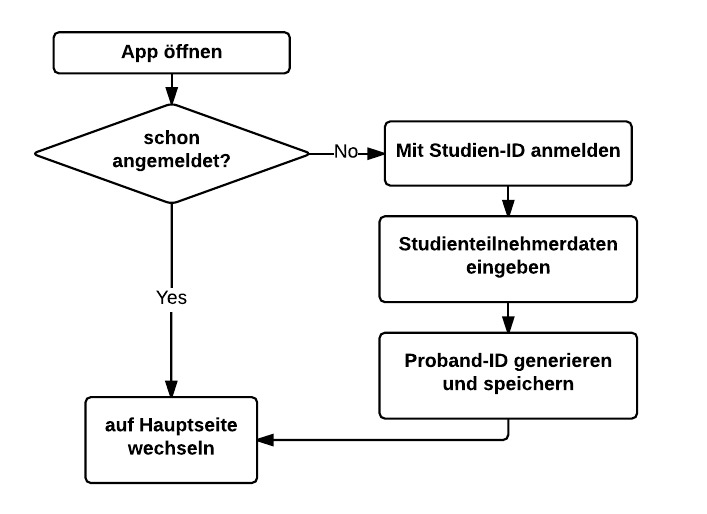
\includegraphics[scale=1]{AppAnmelden.jpeg}
					\caption{Anmelden der Probanden}
				\end{figure}
								

            \item \textbf{/F70/Antworten eines Fragebogens}

            	\par \textbf{Ziel: }Sammeln der Antworten auf den Fragebogen
            	\par \textbf{Vorbedingung: }Anmeldung und mindestens ein vorliegender Fragebogen in der App
            	\par \textbf{Nachbedingung: }die Antworten werden lokal gespeichert
            	\par \textbf{Akteure: }Proband
            	\par \textbf{Auslösendes Ereignis: }Proband erhaltet Notifikation
            	\par \textbf{Beschreibung: }
            	\par 1. Wenn der Versuchsleiter einen Fragebogen sendet, schickt die App eine Notifikation.
            	\par 2. Nachdem der Proband sich angemeldet hat, liegt die App auf der Hauptseite mit einer Liste der auszufüllenden Fragebögen. Der Proband wählt einen Fragebogen aus und beantwortet alle darauf stehenden Fragen. Im Anschluss klickt der Proband auf ``Send'' und die Antworten werden lokal gespeichert.
            	\par \textbf{Alternativen: }
            	\begin{figure}[ht]
            		% \raggedleft
            		\centering
            		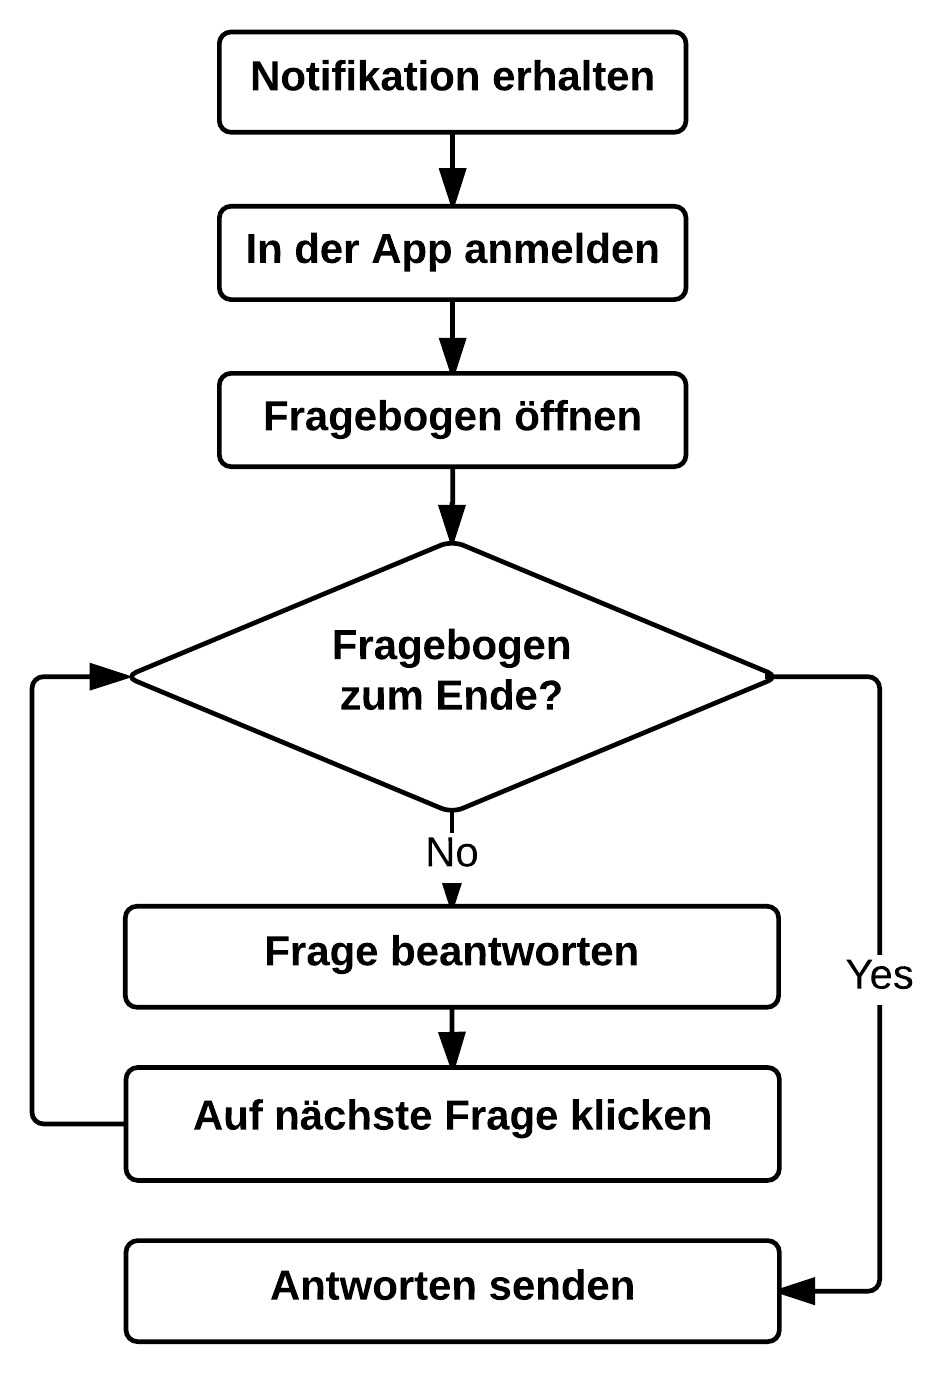
\includegraphics[scale=0.5]{AppAntworten.jpeg}
            		\caption{Antworten eines Fragebogens}
            	\end{figure}
            	

            \item \textbf{/F80/Versenden der Antworten eines Fragebogens}

            \par \textbf{Ziel: }Versenden der Antworten an den Server
            \par \textbf{Vorbedingung: }die Antworten werden lokal gespeichert
            \par \textbf{Nachbedingung (Erfolg): }die Antworten werden auf dem Server gespeichert
            \par \textbf{Nachbedingung (Fehlschlag): }die Antworten werden nicht auf dem Server gespeichert
            \par \textbf{Akteure: }App und Server
            \par \textbf{Auslösendes Ereignis: }die Netzwerkverbindung ist verfügbar und es gibt lokal gespeicherte Antworten
            \par \textbf{Beschreibung: }
            \par Wenn die Netzwerkverbindung vorhanden ist, schickt die App die verfügbaren Antworten an den Server und die Antworten werden auf dem Server gespeichert.
            \par \textbf{Alternativen: }
            \begin{figure}[ht]
            	% \raggedleft
            	\centering
            	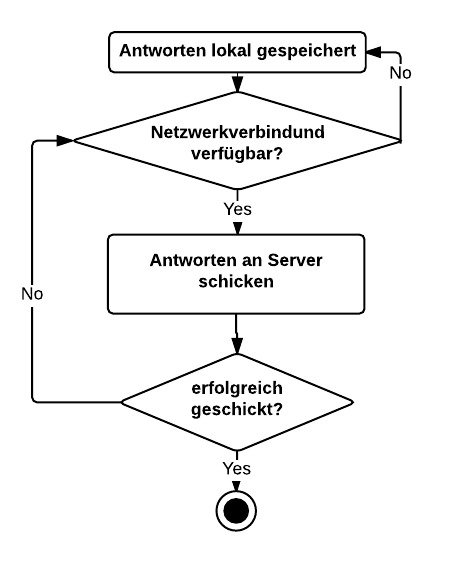
\includegraphics[scale=1.2]{AppVersenden.jpeg}
            	\caption{Versenden der Antworten eines Fragebogens}
            \end{figure}


            \item \textbf{(Wunsch) /F1--/ Sehen der eigenen Antwortquote\footnote{Antwortquote: der Quotient aus beantworteten Fragen und allen Fragen. (Die Antwortquoten sind also für jeden Proband unterschiedlich.)}}

            \par \textbf{Ziel: }Proband kann im Laufen des Versuchs sehen, ob er so viele Fragen wie erforderlich beantwortet hat
            \par \textbf{Vorbedingung: }Proband hat in der App angemeldet
            \par \textbf{Nachbedingung (Erfolg): }die App zeigt die eigene Antwortquote des Probanden
            \par \textbf{Nachbedingung (Fehlschlag): }keine Antwortquote wird gezeigt
            \par \textbf{Akteure: }Proband selbst
            \par \textbf{Auslösendes Ereignis: }Proband klickt auf “My Answer Rate” in der App
            \par \textbf{Beschreibung: }
                \begin{enumerate}
                    \item Bei Erstellen eines Fragebogens kann der Versuchsleiter eine “Bestehensgrenze” der Antwortquote bestimmen. Ein Proband braucht also mindestens eine bestimmte Menge von Fragen beantworten, um die Vergütung am Ende zu bekommen. Die Standardbestehensgrenze liegt bei 60\%.
                    \item Die Bestehensgrenze und die eigene aktuelle Antwortquote wird nicht in der App gezeigt. Gezeigt wird nur, ob man momentan “besteht” oder “nicht besteht”. Man sieht also keine exakte Zahl.
                    \item Im Laufen des Versuchs wird diesen Status stets aktualisiert. Der Proband kann den eigenen Status immer nachsehen.
                    \item Am Ende eines Versuchs kann der Proband das Smartphone zum Versuchsleiter zeigen. Der Versuchsleiter sieht auf dem Smartphone keinen Proband-ID oder genaue Antwortquote, sondern nur “bestanden” oder “nicht bestanden”. So kann der Versuchsleiter die Vergütung entsprechend zahlen.
                \end{enumerate}

        \end{itemize}

    \chapter{Produktdaten}
        \section{Versuchsleiterdaten}
            \begin{itemize}
                \item /D10/ Über einen Versuchsleiter sind folgende Daten zu speichern:
                    \par Name (Anrede, Titel, Vorname, Nachname), Mailadresse (als Kontonummer im System)

                \item /D20/ Macht ein Versuchsleiter Versuche, dann sind folgende Daten zu speichern:
                    \par Versuchsummern der zum Versuchsleiter gehörten Versuchen
            \end{itemize}

        \section{Probanddaten}
            \begin{itemize}
                \item /D30/ Über einen Proband sind folgende Daten zu speichern:
                    \par Proband-ID, Geburtsdatum, Beruf, Geschlecht, Versuchsnummer des daran beteiligten Versuchs

                \item /D40/ Hat ein Proband im Versuch Fragen beantwortet, dann sind folgende Daten zu speichern:
                    \par Antwortquotienten
            \end{itemize}

        \section{Versuchsdaten}
            \begin{itemize}
                \item /D50/ Über einen Versuch sind folgende Daten zu speichern:
                    \par Versuchsnummer, Versuchsname, Anfangs- und Endedatum, “Bestehensgrenze” des Antwortquotienten für die Probanden\footnote{Siehe funktionale Anforderungen F1--}, Mailadresse der Versuchsleiter

                \item /D60/ Hat ein Versuch Probanden, dann sind folgende Daten zu speichern:
                    \par Proband-IDs

                \item /D70/ Hat ein Versuch Fragen, dann sind folgende Daten zu speichern:
                    \par Fragenummer der Fragen
            \end{itemize}

        \section{Fragendaten}
            \begin{itemize}
                \item /D80/ Über eine Versuchsfrage sind folgende Daten zu speichern:
                    \par Fragenummer, Fragetyp, Inhalt der Frage, Versuchsnummer des zugehörigen Versuchs

                \item /D90/ Wird eine Frage im Versuch erscheinen, dann sind folgende Daten zu speichern:
                    \par Erscheinungsereignisse, Abgabetermin

                \item /D100/ Wird eine Frage von Probanden beantwortet, dann sind folgende Daten zu speichern:
                    \par Proband-IDs der Antwortgeber, Abgabezeit der Antworten, Inhalt der Antworten
            \end{itemize}

   \chapter{Nichtfunktionale Anforderungen}
        \begin{itemize}
            \item /NF10/Reaktionszeit

            	\par Die App darf nicht mehr als \_ Sekunden Reaktionszeit haben und die Ladezeit muss unter \_ Sekunden liegen.


        \end{itemize}

        \begin{itemize}
            \item /NF20/Registrierung

            	\par Die Registrierung erfolgt unter Angabe einer E-Mail Adresse und einem Passwort.

        \end{itemize}
        \begin{itemize}
            \item /NF30/Passwort

            	\par Passwörter müssen mindestens 6-stellig sein. Die App kann angemeldet bleiben.


        \end{itemize}
        \begin{itemize}
            \item /NF40/Globalisierung

            	\par Die App ist auf Deutsch und Englisch verfügbar.


        \end{itemize}
        \begin{itemize}
            \item /NF50/Daten speichern

            	\par Die Antworten jedes Fragebogens von den Probanden muss ins Handy gespeichert werden.


        \end{itemize}
        \begin{itemize}
            \item /NF60/Größe der App

            	\par Die App darf nicht mehr als \_ Mb auf dem Handy benötigen.



        \end{itemize}
        \begin{itemize}
            \item /NF70/Integration ins Google Play Store

            	\par Die App soll ins Google Play Store integriert werden.



        \end{itemize}

    \chapter{Benutzungsoberfläche}
    %     Benutzungsoberfläche: grundlegende Anforderungen, Zugriffsrechte
        % \vspace*{1.5cm}
        \subsection{Web-Interface}
            % \vspace*{1.5cm}
            \begin{figure}[ht]
                \centering
                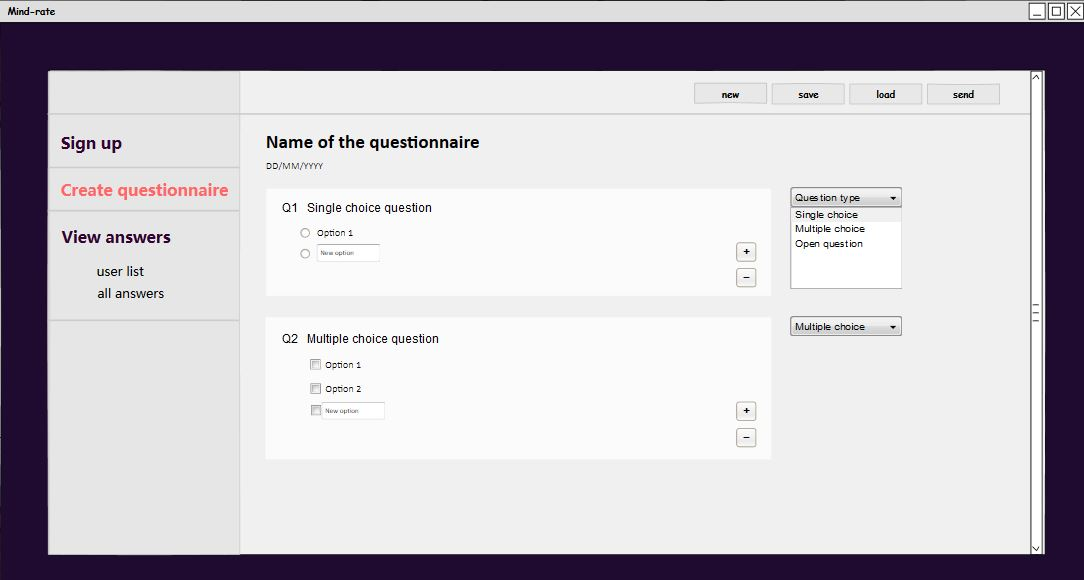
\includegraphics[scale = 0.4]{web.jpg}
                \caption{GUI Entwurf - Web-Interface}
            \end{figure}

            \begin{figure}[ht]
                \centering
                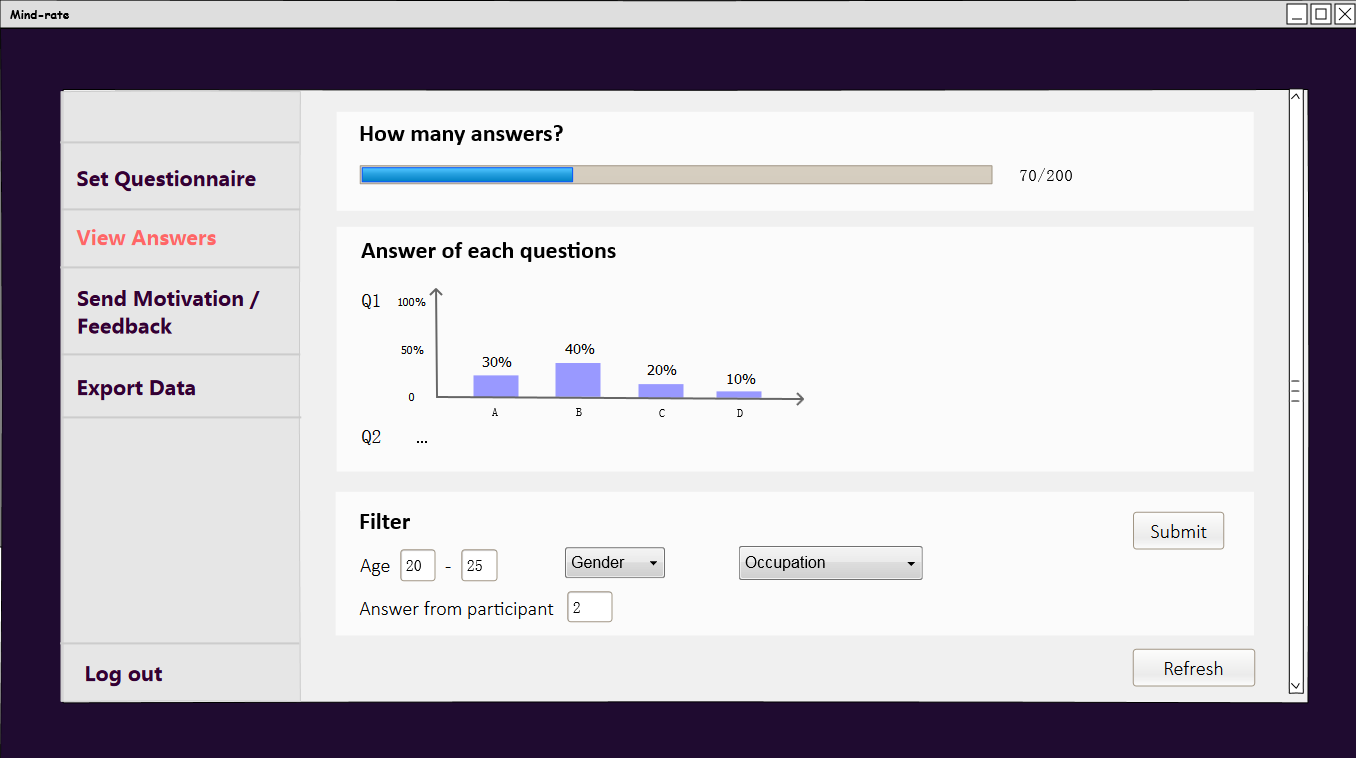
\includegraphics[scale=0.25]{web_ViewAnswer.png}
                \caption{GUI Entwurf - Seite ``View answer''}
                \label{web_ViewAnswer}
            \end{figure}
	
        \newpage
        \subsection{App}
	        \vspace*{2cm}
	        \begin{figure}[ht]
                \centering
                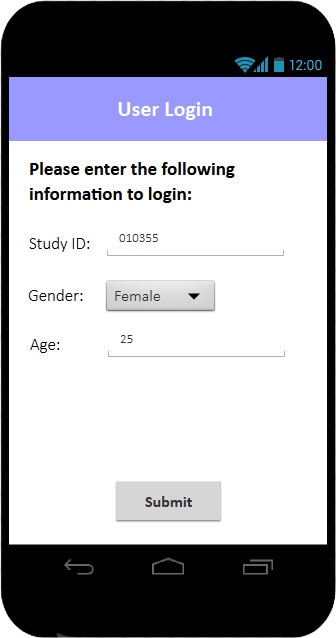
\includegraphics[scale = 0.3]{android_login.jpg}
                \caption{GUI Entwurf - App Login}
            \end{figure}
	
            \vspace*{1cm}
	        \begin{figure}[ht]
                \centering
                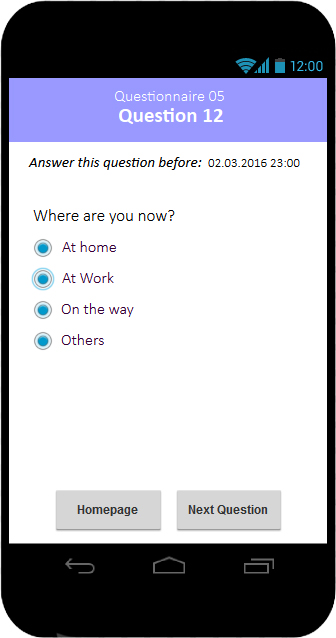
\includegraphics[scale = 0.3]{android_answer.jpg}
                \caption{GUI Entwurf - App Answer Question}
            \end{figure}

    \chapter{Globale Testfälle}

        Folgende Funktionssequenzen sind zu \"uberpr\"ufen:

        \section{Web-Interface}

            \begin{itemize}
                \item \textbf{/TF10/ Registrieren oder Anmelden der Leiter}
	                \begin{itemize}
	                	\item Registrieren:
		                	\begin{enumerate}
			                	\item \par \textbf{Stand: }-keine-
								      \par \textbf{Aktion: }Klicken auf den Button ``Sign Up''
								      \par \textbf{Reaktion: }Werden geleitet zu der Registrieren-Seite
			                	\item \par \textbf{Stand: }Sein in der Registrieren-Seite
							          \par \textbf{Aktion: }Eine Email-Adresse und ein Passwort eingeben
								      \par \textbf{Reaktion: }Eine Bestätigungsmail in dieser Email-Adresse empfangen
			                \end{enumerate}
	                	\item Anmelden:
		                	\begin{enumerate}
		                		\item \par \textbf{Stand: }-keine-
							          \par \textbf{Aktion: }Registrierte Email-Adresse und Passwort eingeben
		                		      \par \textbf{Reaktion: }-keine-
		                		\item \par \textbf{Stand: }Email-Adresse und Passwort übereinstimmen
									  \par \textbf{Aktion: }Klicken auf ``Sign in''
						              \par \textbf{Reaktion: }Sein angemeldet
		                	\end{enumerate}.
	                \end{itemize}

                \item \textbf{/TF20/ Vergessenes Passwort neu zu setzen}
	                \begin{enumerate}
	                	\item \par \textbf{Stand: }-keine-
				              \par \textbf{Aktion: }Klicken auf ``Forgot Passwort'' 
				              \par \textbf{Reaktion: }Werden geleitet zu der Email-Adresse-Eingeben-Seite
	                	\item \par \textbf{Stand: }Sein in der Email-Adresse-Eingeben-Seite
				              \par \textbf{Aktion: }Email-Adresse eingeben
				              \par \textbf{Reaktion: }-keine-
	                	\item \par \textbf{Stand: }Email-Adresse eingegeben
				              \par \textbf{Aktion: }Klicken auf ``Send Email''
				              \par \textbf{Reaktion: }Eine Bestätigungsmail mit einem Link in dieser Email-Adresse empfangen
	                	\item \par \textbf{Stand: }Eine Bestätigungsmail mit einem Link in dieser Email-Adresse empfangen haben
					          \par \textbf{Aktion: }Auf den Link klicken
					          \par \textbf{Reaktion: }Werden zu der Passwort-Setzen-Seite geleitet
	                	\item \par \textbf{Stand: }Sein in der Passwort-Setzen-Seite
				              \par \textbf{Aktion: }Passowort eingeben und ``Reset Passwort'' klicken
					          \par \textbf{Reaktion: }Passwort neu gesetzt
	                \end{enumerate}

                \item \textbf{/TF30/ Verwaltung der Fragen}

	                	\begin{enumerate}
                        \item \par \textbf{Stand: } Der Versuchsleiter ist  angemeldet
                              \par \textbf{Aktion: } Der Versuchsleiter klickt auf ``neu'' Button
                              \par \textbf{Reaktion: }  Der Browser wechselt zur Webseite für die Verwaltung der Fragen

                        \item \par \textbf{Stand: } Webseite für die Verwaltung der Fragen ist geladen
                              \par \textbf{Aktion: } Der Versuchsleiter wählt ``hinzufügen'' im Combobox ``Versuch'' aus
                              \par \textbf{Reaktion: } Ein Dialogfeld ``Versuch 1 erfolgreich hinzugefügt.'' erscheint

                        \item \par \textbf{Stand: } Webseite für die Verwaltung der Fragen ist geladen
                              \par \textbf{Aktion: } Der Versuchsleiter klickt auf ``submit'' Button
                              \par \textbf{Reaktion: } Ein Dialogfeld ``Kein Versuch vorhanden.'' erscheint


                        \item \par \textbf{Stand: } Versuch 1 ist vorhanden
                              \par \textbf{Aktion: } Der Versuchsleiter wählt ``Versuch 1'' im Combobox ``Versuch'' aus
                              \par \textbf{Reaktion: } Der Versuchsleiter kann die konkrete Frage eingeben

                        \item \par \textbf{Stand: } Versuch 1 ist vorhanden
                              \par \textbf{Aktion: } Der Versuchsleiter klickt auf ``submit'' Button
                              \par \textbf{Reaktion: } Ein Dialogfeld ``Keine Frage vorhanden.'' erscheint

                        \item \par \textbf{Stand: } Eine konkrete Frage ist eingegeben
                              \par \textbf{Aktion: } Der Versuchsleiter wählt eine Art im Combobox ``Fragenart'' aus
                              \par \textbf{Reaktion: } Der Versuchsleiter kann die passende Antwortart auswählen

                        \item \par \textbf{Stand: } Eine konkrete Frage ist eingegeben
                              \par \textbf{Aktion: } Der Versuchsleiter klickt auf ``submit'' Button
                              \par \textbf{Reaktion: } Ein Dialogfeld ``Keine Fragenart auswählen.'' erscheint

                        \item \par \textbf{Stand: } Fragenart und Antwortart ist ausgewählt
                              \par \textbf{Aktion: } Der Versuchsleiter klickt auf Checkbox ``Push-Zeit''
                              \par \textbf{Reaktion: } Der Versuchsleiter kann einen Zeitpunkt eingeben (00:00:00-23:59:59)

                        \item \par \textbf{Stand: } Fragenart und Antwortart ist ausgewählt
                              \par \textbf{Aktion: } Der Versuchsleiter klickt auf ``submit'' Button
                              \par \textbf{Reaktion: } Ein Dialogfeld ``Keine Push-Zeit eingeben.'' Erscheint

                        \item \par \textbf{Stand: } Push-Zeit ist eingegeben
                              \par \textbf{Aktion: } Der Versuchsleiter klickt auf Checkbox ``Antwortfrist''.
                              \par \textbf{Reaktion: } Der Versuchsleiter kann einen Zeit eingeben.(eine Zahl eingeben und die Einheit auswählen)


                        \item \par \textbf{Stand: } Antwortfrist ist eingegeben
                              \par \textbf{Aktion: } Der Versuchsleiter klickt auf Checkbox ``Sensor''
                              \par \textbf{Reaktion: } Der Versuchsleiter kann einen Sensor oder mehrere Sensoren hinzufügen.

                        \item \par \textbf{Stand: } Sensor ist aufgestellt
                              \par \textbf{Aktion: } Der Versuchsleiter klickt auf Checkbox ``Vorgesetzte Frage''
                              \par \textbf{Reaktion: } Der Versuchsleiter kann eine vorhandene Frage als die Voraussetzung dieser Frage auswählen

 
                        \item \par \textbf{Stand: } Beziehungen zwischen Fragen ist aufgestellt
                              \par \textbf{Aktion: } Der Versuchsleiter klickt auf ``submit''
                              \par \textbf{Reaktion: } Ein Dialogfeld ``Diese Frage ist erfolgreich hinzugefügt.'' erscheint

                        \item \par \textbf{Stand: } Beziehungen zwischen Fragen ist aufgestellt
                              \par \textbf{Aktion: } Der Versuchsleiter klickt auf ``cancel''
                              \par \textbf{Reaktion: } Alle Aufstellung abtragen

                              
                    \end{enumerate}
	                

                \item \textbf{/TF40/ Antwortsstatus besichtigen}
                    \begin{enumerate}
                        \item \par \textbf{Stand: } Der Versuchsleiter ist noch nicht angemeldet.
                              \par \textbf{Aktion: } Der Versuchsleiter klickt den Button ``View Answers''
                              \par \textbf{Reaktion: } Es wrid zur Anmeldungsseite wechseln.

                        \item \par \textbf{Stand: } Der Versuchsleiter ist angemeldet.
                              \par \textbf{Aktion: } Der Versuchsleiter klickt den Button ``View Answers''
                              \par \textbf{Reaktion: } Der Versuchsleiter kann die \"ubersicht von allen Antwort sehen.

                        \item \par \textbf{Stand: } Der Versuchsleiter bleibt in der Seite ``View Answers''
                              \par \textbf{Aktion: } Der Versuchsleiter klickt den Button ``Refresh''
                              \par \textbf{Reaktion: } Die neue \"ubersicht von allen Antwort wird gezeigt.

                        \item \par \textbf{Stand: } Der Versuchsleiter bleibt in der Seite ``View Answers''
                              \par \textbf{Aktion: } Der Versuchsleiter gibt einige Bedingungen ein und klickt er den Button ``Confirm''
                              \par \textbf{Reaktion: } Die Antwort wird gefiltert. Die \"ubersicht von Antwort der Probanden, die alle eingegebene Bedingungen erf\"ullen, wird geladen.\"ubersicht
                    \end{enumerate}
                    % \begin{itemize}
                    %     \item Durch Klicken von Button ``View answers'' in der linke Men\"u siehe der Versuchsleiter die \"Ubersicht von allen Antwort des aktuellen Fragebogens. \\
                    %     (Abbildung \ref*{web_ViewAnswer})
                    %     \item Durch Klicken von Button ``Refresh'' wird die neuese \"Ubersicht geladen.
                    %     \item Nach Eingeben von verschiedenene Kriterien wird die \"Ubersicht von Antwort der bestimmten Probanden gezeigt.
                    % \end{itemize}

                \item \textbf{/TF45/ Feedback (Motivation) senden}

                    \begin{enumerate}
                        \item \par \textbf{Stand: } Der Versuchsleiter ist noch nicht angemeldet.
                              \par \textbf{Aktion: } Der Versuchsleiter klickt den Button ``Send Motivation / Feedback''
                              \par \textbf{Reaktion: } Es wrid zur Anmeldungsseite wechseln.
                        \item \par \textbf{Stand: } Der Versuchsleiter ist angemeldet.
                              \par \textbf{Aktion: }  Der Versuchsleiter klickt den Button ``Send Motivation / Feedback''
                              \par \textbf{Reaktion: } Der Versuchsleiter wird zur Seite hergeleitet, wo er Motivation / Feedback schreiben und senden kann.
                        \item \par \textbf{Stand: } Der Versuchsleiter bleibt in der Seite ``Send Motivation / Feedback''
                              \par \textbf{Aktion: } Der Versuchsleiter hat die Motivation fertig geschrieben und klickt er den Button ``send''.
                              \par \textbf{Reaktion: } Die Smartphone von Proband erh\"alt eine Notifikation. Durch Klicken von dieser Notifikation kann der Proband die Motivation sehen.
                        % \item \par \textbf{Stand: }
                        %       \par \textbf{Aktion: }
                        %       \par \textbf{Reaktion: }
                        % \item \par \textbf{Stand: }
                        %       \par \textbf{Aktion: }
                        %       \par \textbf{Reaktion: }
                    \end{enumerate}


                    % \par Durch Klicken von Button ``Send Motivation / Feedback'' sieht der Versuchsleiter die Seite, wo er Motivation und Feedback schreiben und senden kann.
                    % \par Durch Klicken von Button ``send'' wird die geschriebene Motivation zu allen Probanden gesandt.
                    % \par Die Smartphone von Proband erh\"alt eine Notifikation. Durch Klicken von dieser Notifikation kann der Proband die Motivation sehen.

                \item \textbf{/TF50/ Exportieren von Daten}
                \begin{itemize}
                	\item \par \textbf{Stand: }Sein angemeldet
			              \par \textbf{Aktion: }Klicken auf ``Export data''
			              \par \textbf{Reaktion: }Daten sind exportiert
                \end{itemize}


            \end{itemize}


        \vspace*{2cm}
        \section{Android-Anwendung}

			\begin{itemize}

            \item \textbf{/TF60/ Anmelden der Probanden}
            \begin{enumerate}
            	\item \par \textbf{Stand: } 
            	\par \textbf{Aktion: }
            	\par \textbf{Reaktion: }
            \end{enumerate}
            
            \item \textbf{/TF--/ Zeigen einer bestandenen Antwortquote}
            \begin{enumerate}
                \item \par \textbf{Stand: }Die Bestehensgrenze der Antwortquote liegt bei 60\%. Der Proband bekommt 10 Fragen.
                \par \textbf{Aktion: }Der Proband beantwortet 6 Fragen, dann klickt auf “My Response Rate”.
                \par \textbf{Reaktion: }Die App zeigt “Momentan sind Sie bestanden. Sehr schön! Bitte weiter machen!”
            \end{enumerate}
            
            \item \textbf{/TF--/ Zeigen einer nicht bestandenen Antwortquote}
            \begin{enumerate}
                \item \par \textbf{Stand: }Die Bestehensgrenze der Antwortquote liegt bei 60\%. Der Proband bekommt 10 Fragen.
                \par \textbf{Aktion: }Der Proband beantwortet 5 Fragen, dann klickt auf “My Response Rate”.
                \par \textbf{Reaktion: }Die App zeigt “Momentan sind Sie nicht bestanden. Kein Problem! Bitte einfach verbessern!”
            \end{enumerate}
        
		    \end{itemize}

    \chapter{Systemmodelle}

        \section{Szenarien}

        \section{Anwendungsf\"alle}

            \subsection{Anwendungsfalldiagramm}
                \vspace{0.4cm}
                \begin{figure}
                    \centering
                    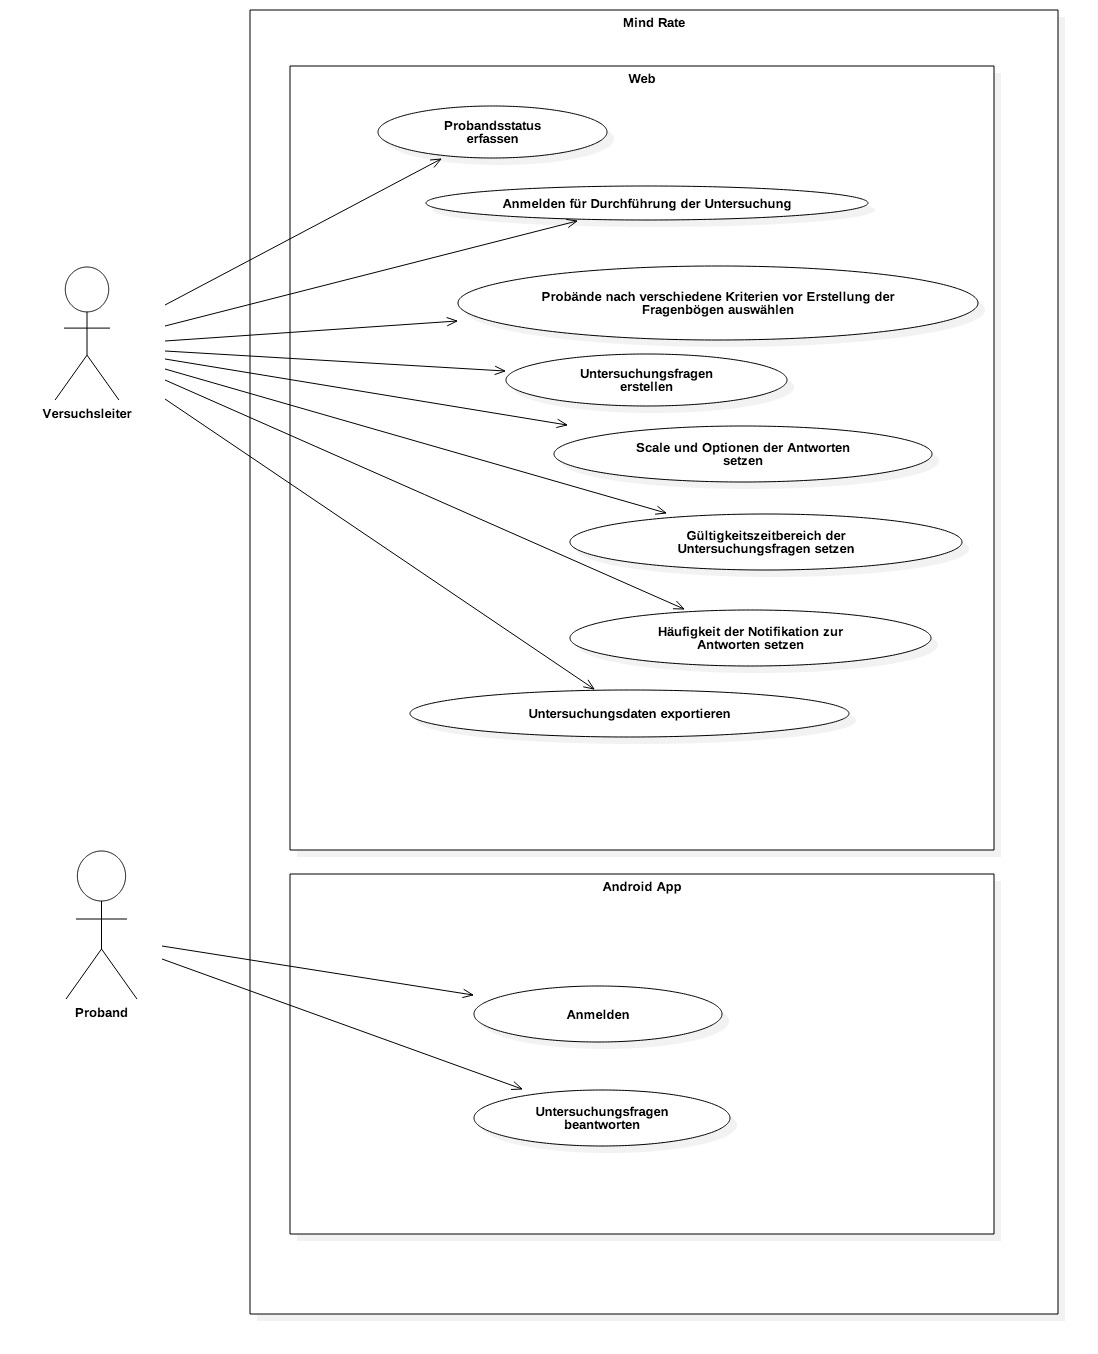
\includegraphics[scale = 0.4]{UseCaseDiagram1.jpg}
                    \caption{Anwendungsfalldiagramm}
                \end{figure}

%    \chapter{Qualitätsziele}
%        Qualiätsziele: Allgemeine Ziele sind meistens Änderbarkeit und Wartbarkeit.
%        Ziele sollten jedoch grundsätzlich messbar, spezifisch und relevant sein.

    \glsaddall
    \printglossaries

    % Abbildungsverzeichnis
    \listoffigures

\end{document}
